\documentclass{standalone}
\usepackage{pgfplots}
\pgfplotsset{compat=newest}
\begin{document}
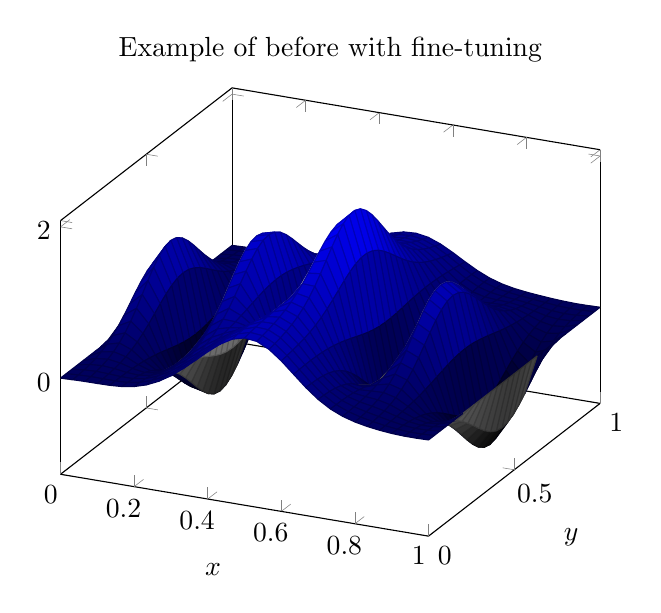
\begin{tikzpicture}
\begin{axis}[
	title=Example of before with fine-tuning,
	xlabel=$x$,
	ylabel=$y$]
\addplot3[surf,
  mesh/interior colormap=
    {blueblack}{color=(black) color=(blue)},
  % slightly increase sampling quality (was 25):
  samples=31,    
  % avoids overshooting corners:
  miter limit=1, 
  % move boundary between inner and outer:
  mesh/interior colormap thresh=0.1,
  colormap/blackwhite, 
  domain=0:1] 
	{sin(deg(8*pi*x))* exp(-20*(y-0.5)^2) 
	+ exp(-(x-0.5)^2*30 
		- (y-0.25)^2 - (x-0.5)*(y-0.25))};
\end{axis}
\end{tikzpicture}
\end{document}
